\documentclass[oneside,final,12pt]{extarticle} %размер бумаги устанавливаем А4, шрифт 12пунктов
\usepackage[utf8]{inputenc}
\usepackage[T2A]{fontenc}
\usepackage[english,russian]{babel}%используем русский и английский языки с переносами
\usepackage{vmargin}
\setpapersize{A4}
\setmarginsrb{26mm}{10mm}{8mm}{8mm}{0pt}{0mm}{0mm}{17mm}
\usepackage{indentfirst}
\sloppy
\usepackage{graphicx} %хотим вставлять в диплом рисунки?
\usepackage{amssymb,amsfonts,amsmath,mathtext,cite,enumerate,float} %подключаем нужные пакеты расширений
\usepackage{titlesec} %хотим вставлять в диплом рисунки?

\begin{document}



\begin{figure}
\quad 1.\quad Перейходим по ссылке https://www.virtualbox.org. Нажимаем кнопку “Download”, выбираем «Windows hosts» и устанавливаем «VirtualBox». 
		
		\centering
		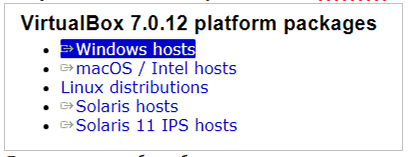
\includegraphics[width=0.65\linewidth]{img/1.png}
\caption{«Windows hosts».}
\label{ris:image}
\end{figure}

\begin{figure}
\quad 2.\quad Далее, для того чтобы любая виртуальная машина могла работать, необходимо включить виртуализацию. Чтобы проверить, включена ли она у вас, откройте диспетчер задач и перейдите в раздел «Производительность». Откройте окно диспетчера задач на весь экран и внизу вы увидите, включена ли виртуализация.

		\centering
		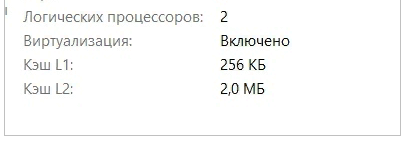
\includegraphics[width=0.65\linewidth]{img/2.png}
\caption{Диспетчер задач. Виртуализация.}
\label{ris:image}
\end{figure}

\begin{figure}
\quad Если виртуализация у вас выключена, то вам необходимо войти в BIOS. Для этого нужно нажать на кнопку «Перезагрузить компьютер», и, как только он начинает запускаться, зажать клавишу «Esc» ( или начать нажимать много раз на клавишу delete, пока не запустится «Startup menu». Зависит от того, ноутбук у вас или компьютер), после чего и откроется «Startup menu». Чтобы открыть BIOS нажмите клавишу «F10». Перейдите в «System Configuration» нажав два раза на кнопку со стрелочкой вправо. Затем спуститесь до «Virtualization Technology», нажав на кнопку со стрелочкой вниз и нажмите клавишу «Enter». Выберите «Enable» и снова нажмите «Enter». Нажмите клавишу «F10» и выберите «Yes». После чего компьютер перезагрузится уже с включённой виртуализацией.

		\centering
		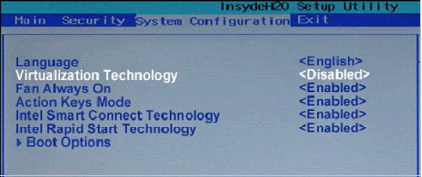
\includegraphics[width=0.65\linewidth]{img/3.png}
\caption{BIOS. «Virtualization Technology».}
\label{ris:image}
\end{figure}

\begin{figure}
3. Скачиваем «Ubuntu» с официального сайта по ссылке: https://ubuntu.com/download/desktop. Затем открываем «VirtualBox» и нажимаем кнопку «Создать». Заполняя все поля, необходимо указать объём памяти не менее 2 гигабайт, иначе «Ubuntu» просто не запустится. В остальном можно принять все установки по умолчанию. После создания, необходимо нажать на кнопку «Настройки», далее «Носители», у надписи «Контроллер: IDE» нажать на значок диска с плюсиком. 

		\centering
		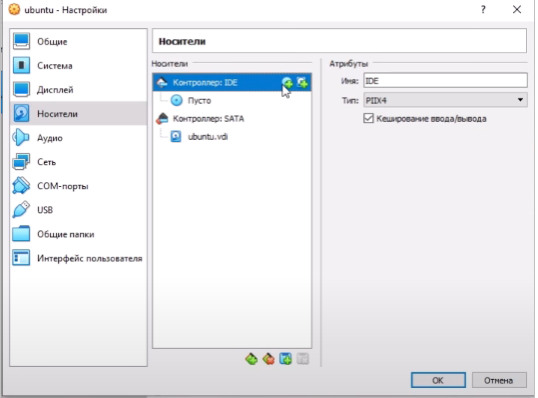
\includegraphics[width=0.65\linewidth]{img/4.png}
\caption{Настройки. Носители.}
\label{ris:image}

\end{figure}

\begin{figure}
\quad Затем «Добавить» и выбрать скаченный ранее файл с «Ubuntu». После чего можно нажать кнопку «Запустить». После запуска, мы выбираем язык, нажимаем скачать «Ubuntu», заполняем все поля, и выбираем параметры по умолчанию. И наконец видим интерфейс «Linux».
\end{figure}

\end{document}
